
\begin{figure}[!htp]
    \centering
    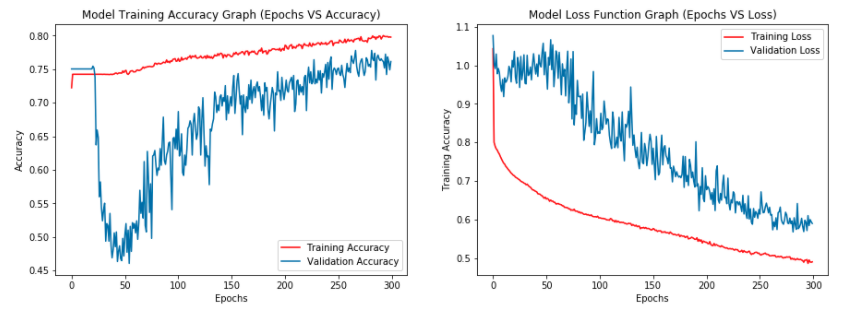
\includegraphics[width=\textwidth]{Images/iConv.png}
    \caption{Convolutional Neural Network}
    \label{fig:cnn}
\end{figure}

The model architecture was changed with increase of four more convolutional layers in the network
to detect more feature maps from images. The additional convolutional layers contains filters of 128 and 256 
respectively.Furthermore, the model was trained for three hundred epochs with validation 
data to adjust the weights and improve the accuracy of the model with learning rate of 0.001 using SGD optimiser from the 
above experiments. The figure \ref{fig:cnn} shows the graph of increase in model accuracy of training and 
validation data over three hundred epochs. Furthermore, the diagram also shows the decline in the 
loss or cost function of the model. The model was evaluated on the testing data and resulted in 77.4 \% accuracy
in detecting the pigmented skin lesions. \footnote{\url{https://github.coventry.ac.uk/sareenv/Final-Year-Project/blob/master/Research}}
\pagebreak
\subsubsection{Model Training without validation data}
\begin{figure}[!htp]
    \centering
    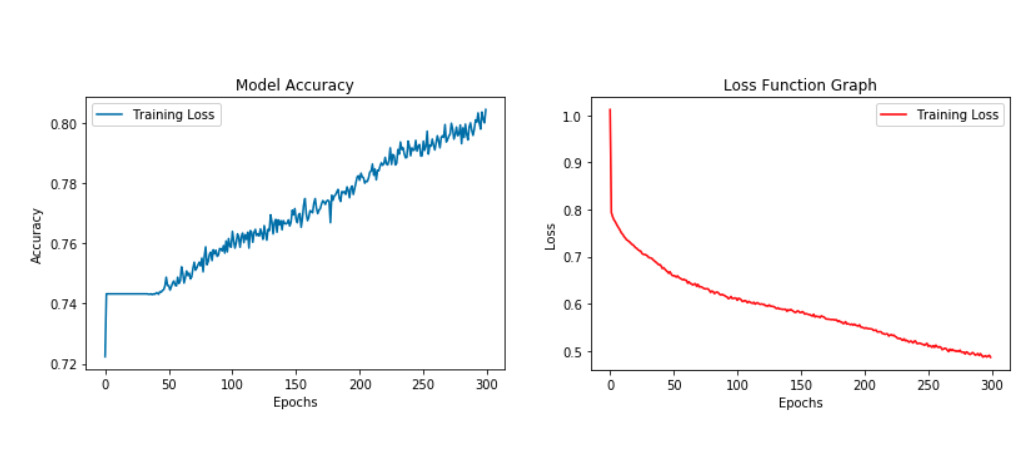
\includegraphics[width=\textwidth]{Images/wvalid.png}
    \caption{Model training without validation data}
    \label{fig:cnnwvalid}
\end{figure}
The experiment was performed with the same model architecture as above without providing the validation 
data to the model. The figure \ref{fig:cnnwvalid} show the increase in the model accuracy and decline in the 
the loss function over three hundred epochs.The accuracy of the model was evaluated to be 74.39\% on testing data. 
Therefore, the further model experiments were performed with validation data. 